\section{Variando e inventando}


É importante variar o estilo do slide para criar apresentações mais dinâmicas.

Isso é bem fácil no \textit{Power Point}, porém é mais difícil no \texttt{beamer}, que exige certa prática de \LaTeX\  para sair dos formatos mais padronizados. Porém, isso é tão fácil no \textit{Power Point} que muitos usuários abusam, criando slides confusos ou fora do padrão de uso, isto é, sem usar as caixas de conteúdo, o que dificulta a mudança de estilo.


A Figura \ref{fig:man} mostra um slide bem diferente do que os apresentados normalmente, mas ainda em um formato ``retangular''. Já a Figura \ref{fig:formulas} mostra uma derivação de uma fórmula em um formato diferente, incluindo um gráfico. A Figura \ref{fig:tres} também mostra como um tema foi tratado com vários slides diferentes, cada um com um formato.

Use os formatos para tirar a monotonia da aula. Use também animações nos slides, mas cuidado com as transições entre os slides, que devem ser usadas muito parcimoniosamente, porque quebram a atenção.

\begin{figure}[htb]
    \centering
    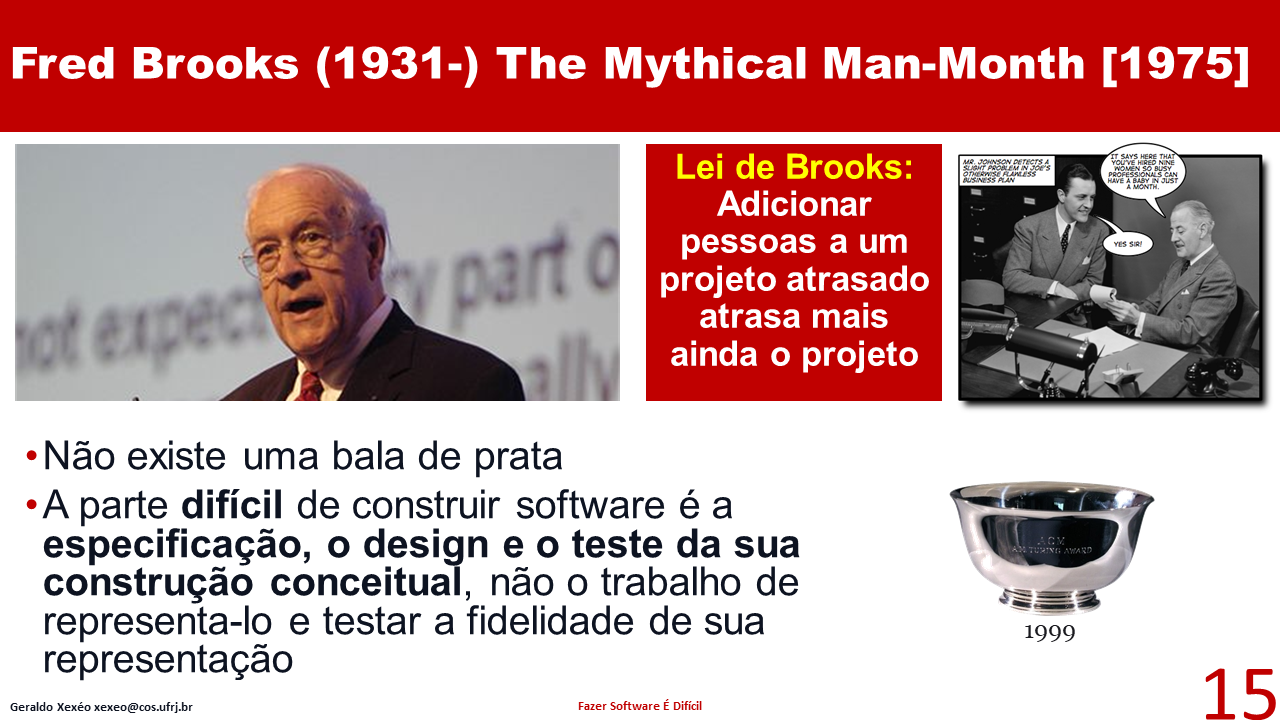
\includegraphics[width=\tam\linewidth,frame]{imagens/manmonth.png}
    \caption{Um slide com um formato diferente}
    \label{fig:man}
\end{figure}

Os slides não devem ser exagerados, nem em texto, nem em decoração, porém um ou outro slide pode ser mais divertido, ou mais pesado em texto.


Em um slide com fórmulas, como o da Figura \ref{fig:formulas}, elas devem aparecer uma a uma se estiverem sendo calculadas. Se for apenas um comentário sobre a complexidade das fórmulas, que você deseje passar por cima em busca de uma explicação mais fácil, elas podem aparecer todas de uma vez.

\begin{figure}[hbt]
    \centering
    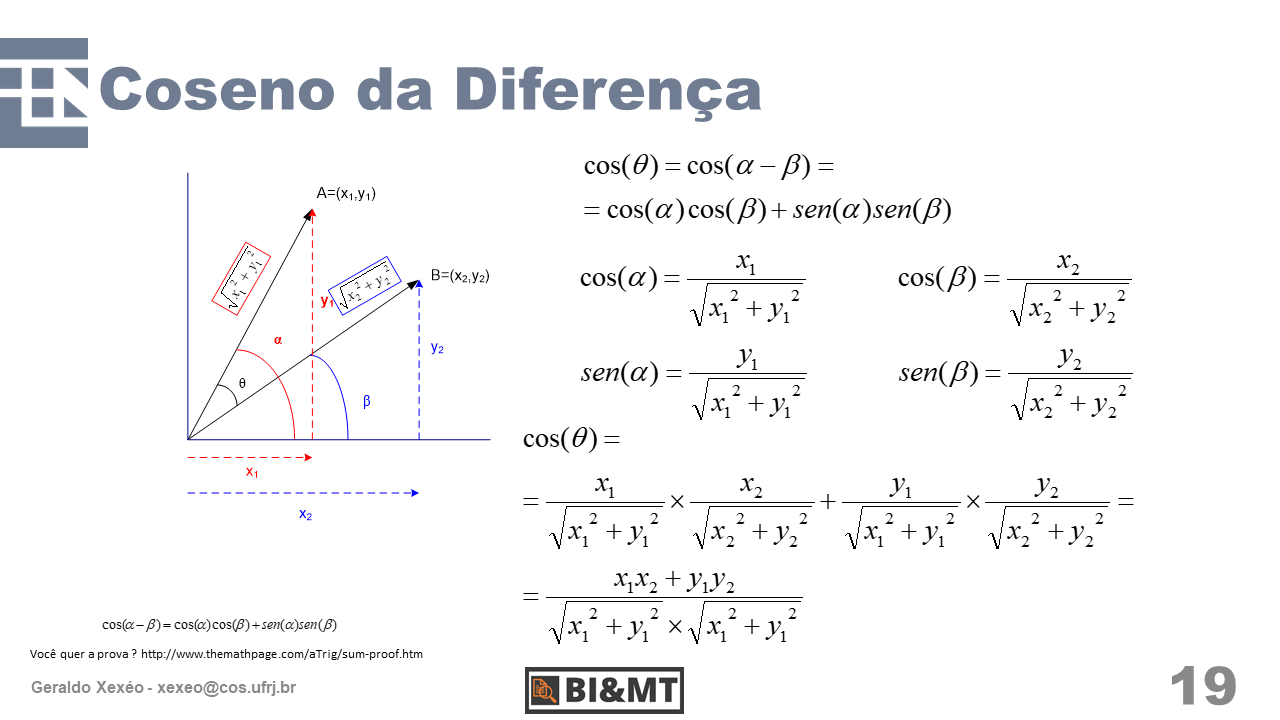
\includegraphics[width=\tam\linewidth,frame]{imagens/desenhoeformulas.png}
    \caption{Desenho e fórmulas em um slide, que possui o logo do laboratório ligado ao curso e um logo que foi criado para identificar o curso em 3 lugares: Moodle, Whatsapp e GitHub.}
    \label{fig:formulas}
\end{figure}



Slides ``divertidos'', como os que estão resumidos\footnote{Esses slides foram encontrados em     \url{https://unblast.com/funtastic-free-powerpoint-presentation-template-ppt/}
} na Figura \ref{fig:fun} vão criar uma carga cognitiva muito grande em uma apresentação e podem incomodar membros de uma banca. Já vi isso acontecer. Mas isso não quer dizer que não possam ser usados em um ou outro slide, como marcos de início de seção ou outra alternativa de menor impacto que usá-los em toda aula. Também podem ser úteis em uma apresentação muito curta, ou em um ambiente de divulgação científica.

\begin{figure}[hbt]
    \centering
    
\includegraphics[width=\tam\linewidth,frame]{imagens/funslide.jpg}
    \caption{Exemplos de slides divertidos.
        (Fonte: unblast.com) }
    \label{fig:fun}
\end{figure}

\subsection{Quebrando as regras}

É possível quebrar as regras algumas vezes para tirar a monotonia das aulas ou para deixar um ponto mais claro.

No slide da Figura \ref{fig:magica} fiz uma brincadeira com a turma, para chamar atenção em meio a uma aula expositiva onde não havia atividades. Para auxiliar a quebrar o ritmo escolhi, apenas nesse slide da aula, usar uma fonte totalmente diferente, que inclusive dificulta  a leitura, mas que tenta simular uma fonte mágica.

\begin{figure}[tbh]
    \centering
    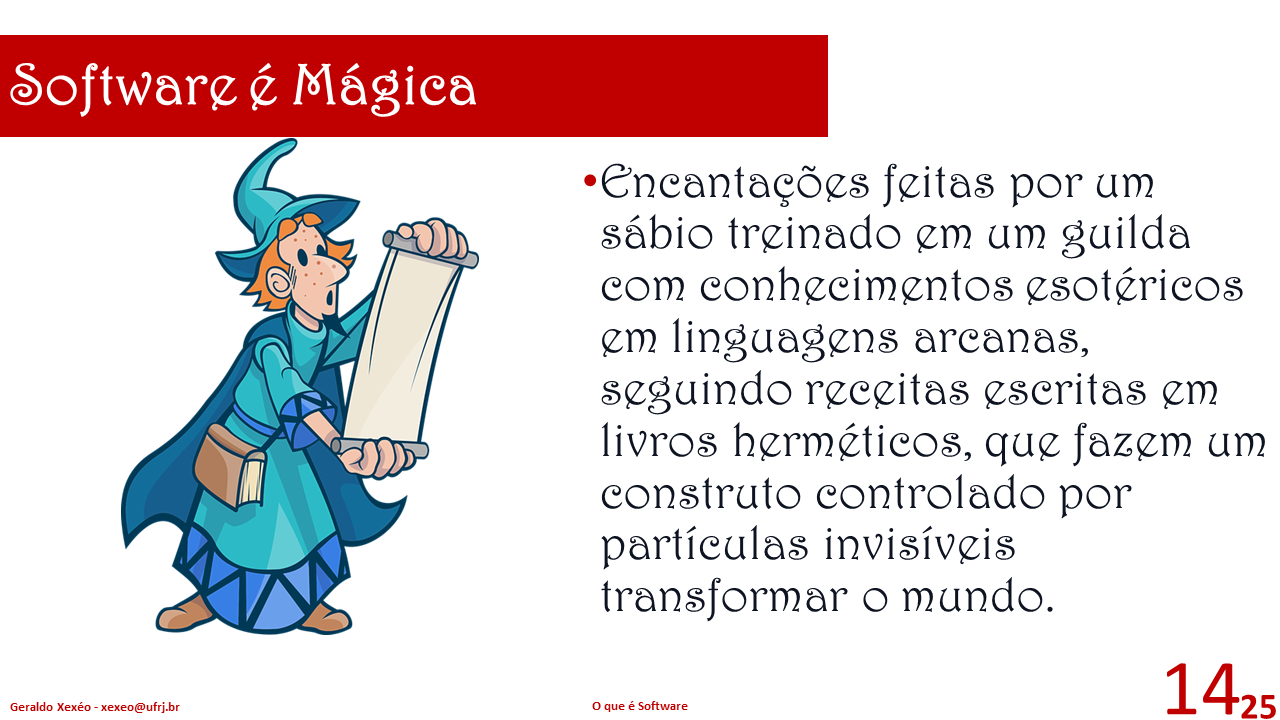
\includegraphics[width=0.7\linewidth]{imagens/magica}
    \caption{Slide feito para ``acordar'' e motivar a turma em uma aula que explica o que é software.}
    \label{fig:magica}
\end{figure}

Já o slide da Figura \ref{fig:ponte} usa a técnica da ``figura inspiradora'', que eu não considero correta para toda uma aula, e também não tem título. Mas ele aparece logo depois de um slide comum que acaba com a sentença ``Um projeto é uma ponte do estado atual para um futuro melhor''. Eu uso o slide para explicar melhor o conceito de por que fazemos projeto, mas ele está lá para motivar e mudar um pouco o tom da aula, até aquele momento com slides de definição e instrução. Nesse momento o slide serve de cenário para os comentários, mas o slide anterior garante que a ideia específica está registrada.

\begin{figure}[tbh]
    \centering
    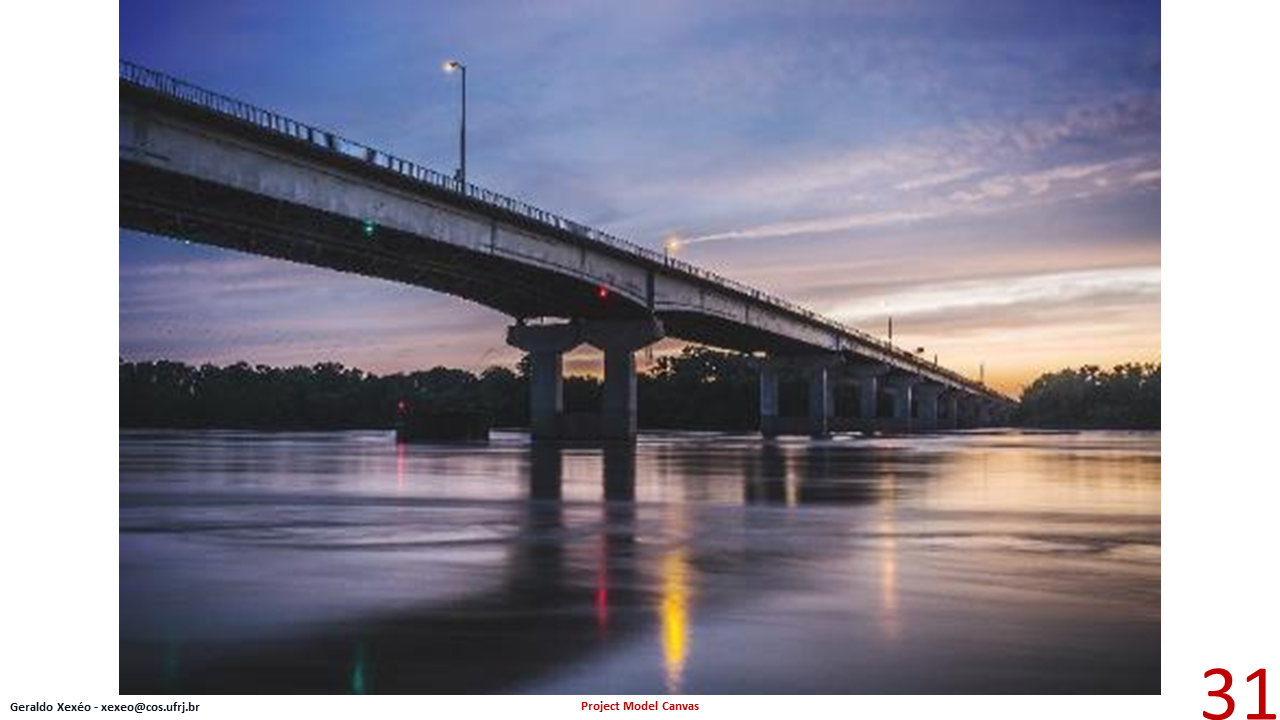
\includegraphics[width=0.7\linewidth,frame]{imagens/ponte}
    \caption{Figura da ponte só aparece porque no slide anterior há a frase ``Um projeto é uma ponte do estado atual para um futuro melhor''}
    \label{fig:ponte}
\end{figure}

